\documentclass[15pt]{article}
\usepackage[]{cite}   % remove to use brackets instead of superscripts in citations
\usepackage{graphicx}
\usepackage{fancyhdr}
\usepackage{xcolor}
\usepackage{indentfirst}
\usepackage[a4paper, portrait, margin=1in]{geometry}
\usepackage{lastpage}
\usepackage{float}
\usepackage{tabularx}
\usepackage{setspace}
\usepackage{csvsimple}
\usepackage{longtable}
\usepackage{wrapfig}
\pagestyle{fancy}
\fancyhf{}
\fancyhead[L]{Vupiter}
\fancyhead[R]{Final Report}
\rfoot{Page \thepage \hspace{1pt} of \pageref*{LastPage}}
\pagenumbering{arabic}
\newcolumntype{L}{>{\centering\arraybackslash}m{3cm}}
\usepackage[pdftex,bookmarks,pdfpagemode=UseOutlines,
    pdfauthor={Vupiter Team},
    pdftitle={Final Report},colorlinks=true, linkcolor=blue]{hyperref}
% removed colorlinks after bookmarks

\newcommand{\code}[1]{\texttt{\smaller #1}}

\setlength\parindent{5ex}
\setlength\parskip{2ex}
\newcommand\xrowht[2][0]{\addstackgap[.5\dimexpr#2\relax]{\vphantom{#1}}}
\newcommand{\fig}[1]{\centerline{\includegraphics{#1}}}

\DeclareGraphicsExtensions{.pdf, .jpg, .png}
%\setkeys{Gin}{width=0.85\textwidth}
\onehalfspacing
\begin{document}
\begin{titlepage}
    \begin{singlespace}
    \begin{center}
        \vspace*{1cm}
            
        \Huge
        \textbf{Vupiter DC Power Supply}
            
        \vspace{0.5cm}
        \large
        Date: \today
            
        \vspace{2.25cm}

        \textbf{Senior Design Mid-term Report}
        
        \vspace{2.25cm}

        \textbf{Team Members:}\\
        Chase Flatau\\
        Alex Jones\\
        Rice Shelley\\
        Al Spies\\
        \textbf{Faculty Advisors:}\\
        Doctor Robert Nelms\\
        Doctor Thadeus Roppel
        \vfill
            
            
        \vspace{0.8cm}
            
        
\includegraphics[width=0.4\textwidth]{university}
            
        \Large

        \textbf{Auburn University}\\
        Department of Electrical and Computer Engineering\\

            
    \end{center}
\end{singlespace}
\end{titlepage}
\section{Executive Summary - Rice Shelley}
The DC power supply is an integral piece of equipment for electronics labs. Often more than one DC power source is required for a project. Electronic test equipment vendors have addressed this issue and provide multichannel DC power supply in the \$300\cite{expensive} and up price range. However, for the electronic hobbyist, this is not always an economically attractive option. Vupiter provides a three-channel DC power supply for around \$100 centered on open-source ideology. The price point of the supply is lowered by allowing users to order PCBs and parts to assemble the power supply themselves. Vupiter’s design flexibility, price point, and ease of use will make it an attractive option for anyone working with electronics. 

Each output is isolated and provides both constant voltage and current modes. The supply can deliver 0–30V at 5A on each channel at a resolution of 10mA / 10mV. Individual channels are controlled with two rotary encoders and an LCD screen as seen in \autoref{fig:fullpic}. In addition to the traditional front panel, a multi-platform virtual interface to the supply is provided. This interface uses SCPI (Standard Commands for Programmable Instruments) enabling simple development of control software, test case automation, and data collection. Vupiter meets all of these target specifications with the one exception of board longevity on the transformer board.

On future iterations of Vupiter multiple improvements can be made. The MCU on the linear board, an EFM8BB3, will be bought in a package more suited to hand soldering. A more convent MCU package will make assembly easier for the average hobbyist. Also on the linear board, replacing the single turn tuning potentiometers with multiturn would make the calibration process easier. The isolation stage could use better demagnetization diode selection and a high bandwidth control loop. The PFC could use improved filtering.

Despite this laundry list of improvements, two of the three boards, the PFC and linear boards, work correctly. The transformer boards break after approximately 30 minutes of use. The transformer board's lifespan could have been improved with better demagnetization diode selection. The power supply per-unit cost ended at \$103, which is right on target and very competitive for a 3 channel supply. None of the redesigns listed above are expected to appreciably increase the cost meaning Vupiter can be a viable contender for any hobbyist.

\begin{figure}[H]
    \begin{center}
      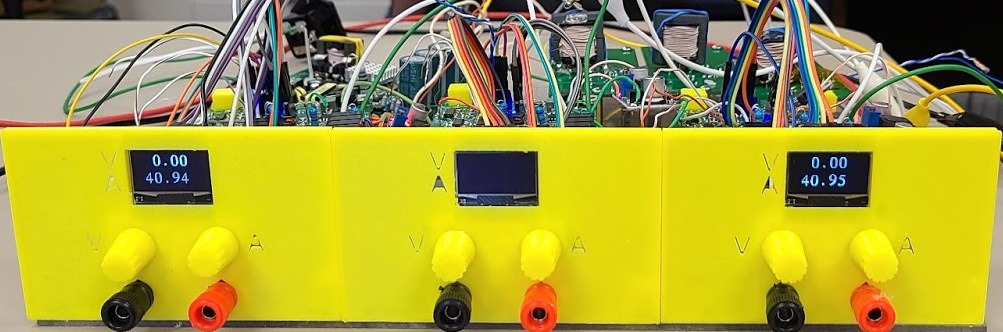
\includegraphics[width=\textwidth]{v}
    \end{center}
    \caption{Vupiter Fully Assembled}
    \label{fig:fullpic}
  \end{figure}
\pagebreak
\begin{singlespace}
    

\tableofcontents
\end{singlespace}
\pagebreak

\section{Introduction - Rice Shelley}
Vupiter DC power supply has three independent isolated channels each with an output of 0 - 30V at 5A and a resolution of 10ma / 10mv. The power supply features a physical front panel as well as a desktop computer interface. The physical front panel allows for normal lab operation, while the virtual front panel can be used for test automation. The virtual front panel will comply with industry standards for interfacing programmable instruments so that preexisitng software may be used with the Vupiter power supply. Vupiter is entirely open source to allow for easy modifications and tailored functionality. Vupiter’s comparatively low cost will provide accessibility for hobbyists and makers. Multi-channel power supplies are typically priced in the \$300 plus range. Vupiter will provide a comparatively affordable option in the 
\$100 range with similar functionality. The price of the supply can be lowered by allowing hobbyist to purchase the PCB’s and parts to assemble the power supply themselves.

\section{Vupiter's Design}
\subsection{Topology - Chase Flatau}
The Vupiter project is a three-channel power supply; therefore, there are three separate lines for each channel. Each channel will be fed from a single Power Factor Correction board before splitting. This is followed by a switched power mode board, a linear power board, and finally a human interface. The first stage is the power supply to our power supply which will be a standard wall outlet leading into the PFC stage. The PFC will take the wall output, 85-265 VAC, and convert it to 400 VDC. Only one of these is needed for the three isolated channels. This in turn leads into the three switch-mode boards. Each of these boards controls their channel and can work independently of the other two. Each one will take the 400 VDC and output 36-6 VDC at a max of 5.5 A. There is a built-in 6 VDC and 0.5 A built-in for the linear stage to use for control.

The next stage is the linear power boards. These boards control the final output of each channel. This is accomplished through op-amps and a microchip controlling BJTs. The maximum output for a single channel is 36 VDC at 5 A. All of this is controlled by a human interface, either through the respective front panel controls or a USB connection to a computer. Each channel will have an OLED screen to display the current settings and its own set of push knobs to control voltage and current. The power supply can also be controlled through a provided GUI or any program that the user may design and send over SCPI(Standard Commands for Programmable Instruments). Due to the open sources used, the user has a large degree of freedom to change what they want to better fit what they need.

Our group decided to use a switch-mode stage leading into a linear stage because of the cost and performance. By utilizing a switch-mode section, Vupiter eliminates expensive 60 Hz transformers that a more classical design would require; the benefit of a linear section, its high-quality output, is retained. This combination of high-quality output and a less expensive design made a mixed-mode supply the most attractive and logical choice.

\begin{figure}[H]
    \centering
    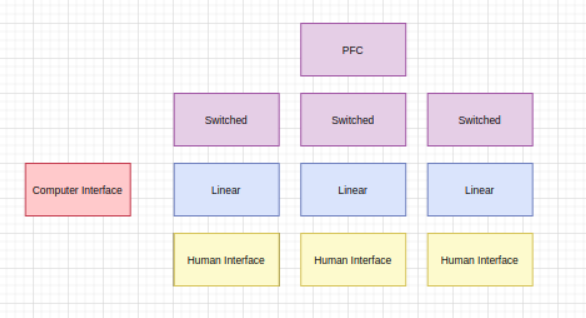
\includegraphics[width=0.6\textwidth]{chase1}
    \caption{Topology of entire supply}
    \label{fig:chase1}
\end{figure}

\subsection{Linear - Chase Flatau}

\subsubsection{Requirements}
\begin{itemize}
\item 36 VDC input \begin{itemize}
    \item This is provided from the switched mode module.
\end{itemize}
\item 30 VDC, 5 A output \begin{itemize}
    \item These were the parameters that were initially decided upon.
\end{itemize}
\item Full Isolation \begin{itemize}
    \item IEC 62368 \cite{5} requires isolation for safety and we chose full isolation for better functionality of our power supply. This applies to the UART interface of this board.
\end{itemize}
\item Printed boards \begin{itemize}
    \item Printed boards will be in compliance with UL 796\cite{796} and shall be classed V-1 or less flammable.
\end{itemize}
\end{itemize}

\subsubsection{Design}


The linear stage can be broken down into five basic sections based on the common ground plane to which they belong The first section is switching components. The two main components in this group are the Switching Regulators, based off the MC33063A, which are used for dc-dc conversion. These regulators provide the 5V and -3V power lines necessary for the analog and digital components used in the rest of the board. The next section is the digital components. This uses a linear regulator to take the five volts from the switching components and regulate it to 3V, which is used to power the microchip that controls the rest of the board.


The last two sections could be considered parts of a whole. These sections, the power and analog control, are comprised of BJTs and op-amps mostly. The power section uses BJTs to regulate the 36 V from the switch-mode supplies to the desired output voltage. To achieve this, op-amps take the feedback from the output of the power section and, along with control lines from the microchip, set the correct voltage to control the BJTs.

\begin{wrapfigure}[30]{r}{0.35\textwidth}
    \begin{center}
      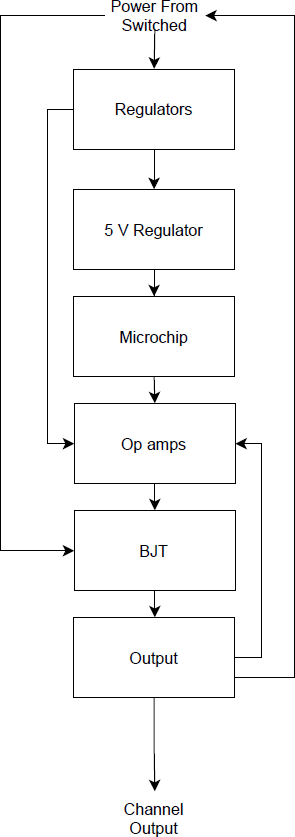
\includegraphics[width=0.33\textwidth]{chase7}
    \end{center}
    \caption{Linear board basic flow}
    \label{fig:chase7}
  \end{wrapfigure}
Throughout the linear stage, ceramic capacitors are preferred as they naturally have a low ESR and generally have a smaller footprint. Most resistors are of a general SMD type with a few notable differences. The resistors at the output on the power section need to be power rated which makes them much larger than a 0805 resistor. There are also several potentiometers used throughout the design which allow greater control for fine-tuning for the regulators and op-amps. Most other parts are standard and can be purchased in large quantities for a relatively cheap price.

We decided to use BJTs instead of MOSFETs or discrete chips such as in \cite{adexpense}because they better fit our needs. We decided against MOSFETs because they have sharp turn-on characteristics and they minimize their linear range. This is not a good choice for a linear board as it can cause unstable oscillations when control loops have high bandwidth. Specialized chips were not a good financial choice because they would drive the cost of a single unit much higher than the \$100 goal we decided upon. 

\subsubsection{Performance}
The first issue that was discovered before testing was an issue with the microcontroller, EFM8BB3. Due to a misunderstanding of the datasheet, we believed there were four Digital to Analog Converters (DACs) available; however, when our programmers were trying to program the chip, they found only two DACs. The easiest solution was to remap the pins and use some paths that were not initially considered.
    
The second issue was discovered during testing and has to do with one of the buck regulators. The chip that was used, MC33063AD, was discovered to be insufficient for the load that the -3 V regulator would place upon it. This issue went unnoticed at first because the testing voltages were so low, 6 V or less, that it wasn’t an issue. Once the voltage was pushed higher and closer to standard operating voltages, the chip was blown. The cause is most likely due to an error in the datasheet. The datasheet bases $L_{min}$ off of $V_{min}$ instead of $V_{max}$ which gives a lower inductance than was necessary for our purposes. This issue was fixed by replacing the regulator with an external buck regulator board that could handle the extra load.

Despite these issues, the linear board works as designed. Some improvements that would be added if we were to redesign the power supply include a negative linear regulator after the -3 V regulator and multi-turn potentiometers. Adding a negative linear regulator would drastically reduce the noise in the linear board and improve its performance. Such an addition would also have a negligible impact on the overall cost of the unit. Switching to multi-turn potentiometers will make it is easier to calibrate the device and therefore improve the overall performance of the linear section of the board.


\pagebreak
\subsection{AC/DC Topology Breakdown - Alex Jones}
The original plan for the AC to DC stage design was a single switch-mode converter per channel to supply voltage transformation and isolation. Ultimately this cannot work, as the linear stage’s need for a variable supply combined with potentially variable AC supply would put impossible duty cycles on the forward converter for any given transformer setup. For example, at the two extremes, we need to support both 85 VAC to 36 VDC and 265 VAC to 6 VDC. The first of these is a ratio of 3:1, while the other is a ratio of 63:1. That level of versatility in a supply is simply impossible due to switching speeds and the need to reset the inductor.

This issue strongly indicates the need for an additional switch mode supply in the chain. This second supply would allow for each converter to have either a fixed input or a fixed output, instead of variable requirements on both. A common choice for this problem is an input power factor correction circuit. Firstly, PFC is required by IEC 61000-3-2 for all consumer devices. Secondly, common PFC topologies increase the total voltage to an intermediary 400 VDC supply. An intermediary voltage is useful as it decreases current stress and inductance requirements on the subsequent forward converter.

Thus, our final topology for the AC to DC converter stage is a boost power factor correction(PFC) circuit followed by a forward converter. This additional converter is an additional layer of complexity but it makes up for it as it acts as a pre-regulator, reducing complexity and stresses on the forward converter, and it helps the total device be standard compliant.  This topology is represented in \autoref{fig:acdctopo}. The topology of a pre-regulator in the form of boost PFC is so common that \emph{The Art of Electronics}\cite{aoe} recognizes the design as a driving market force the development of cheap 600 volt MOSFETs.

\begin{figure}[H]
    \centering
    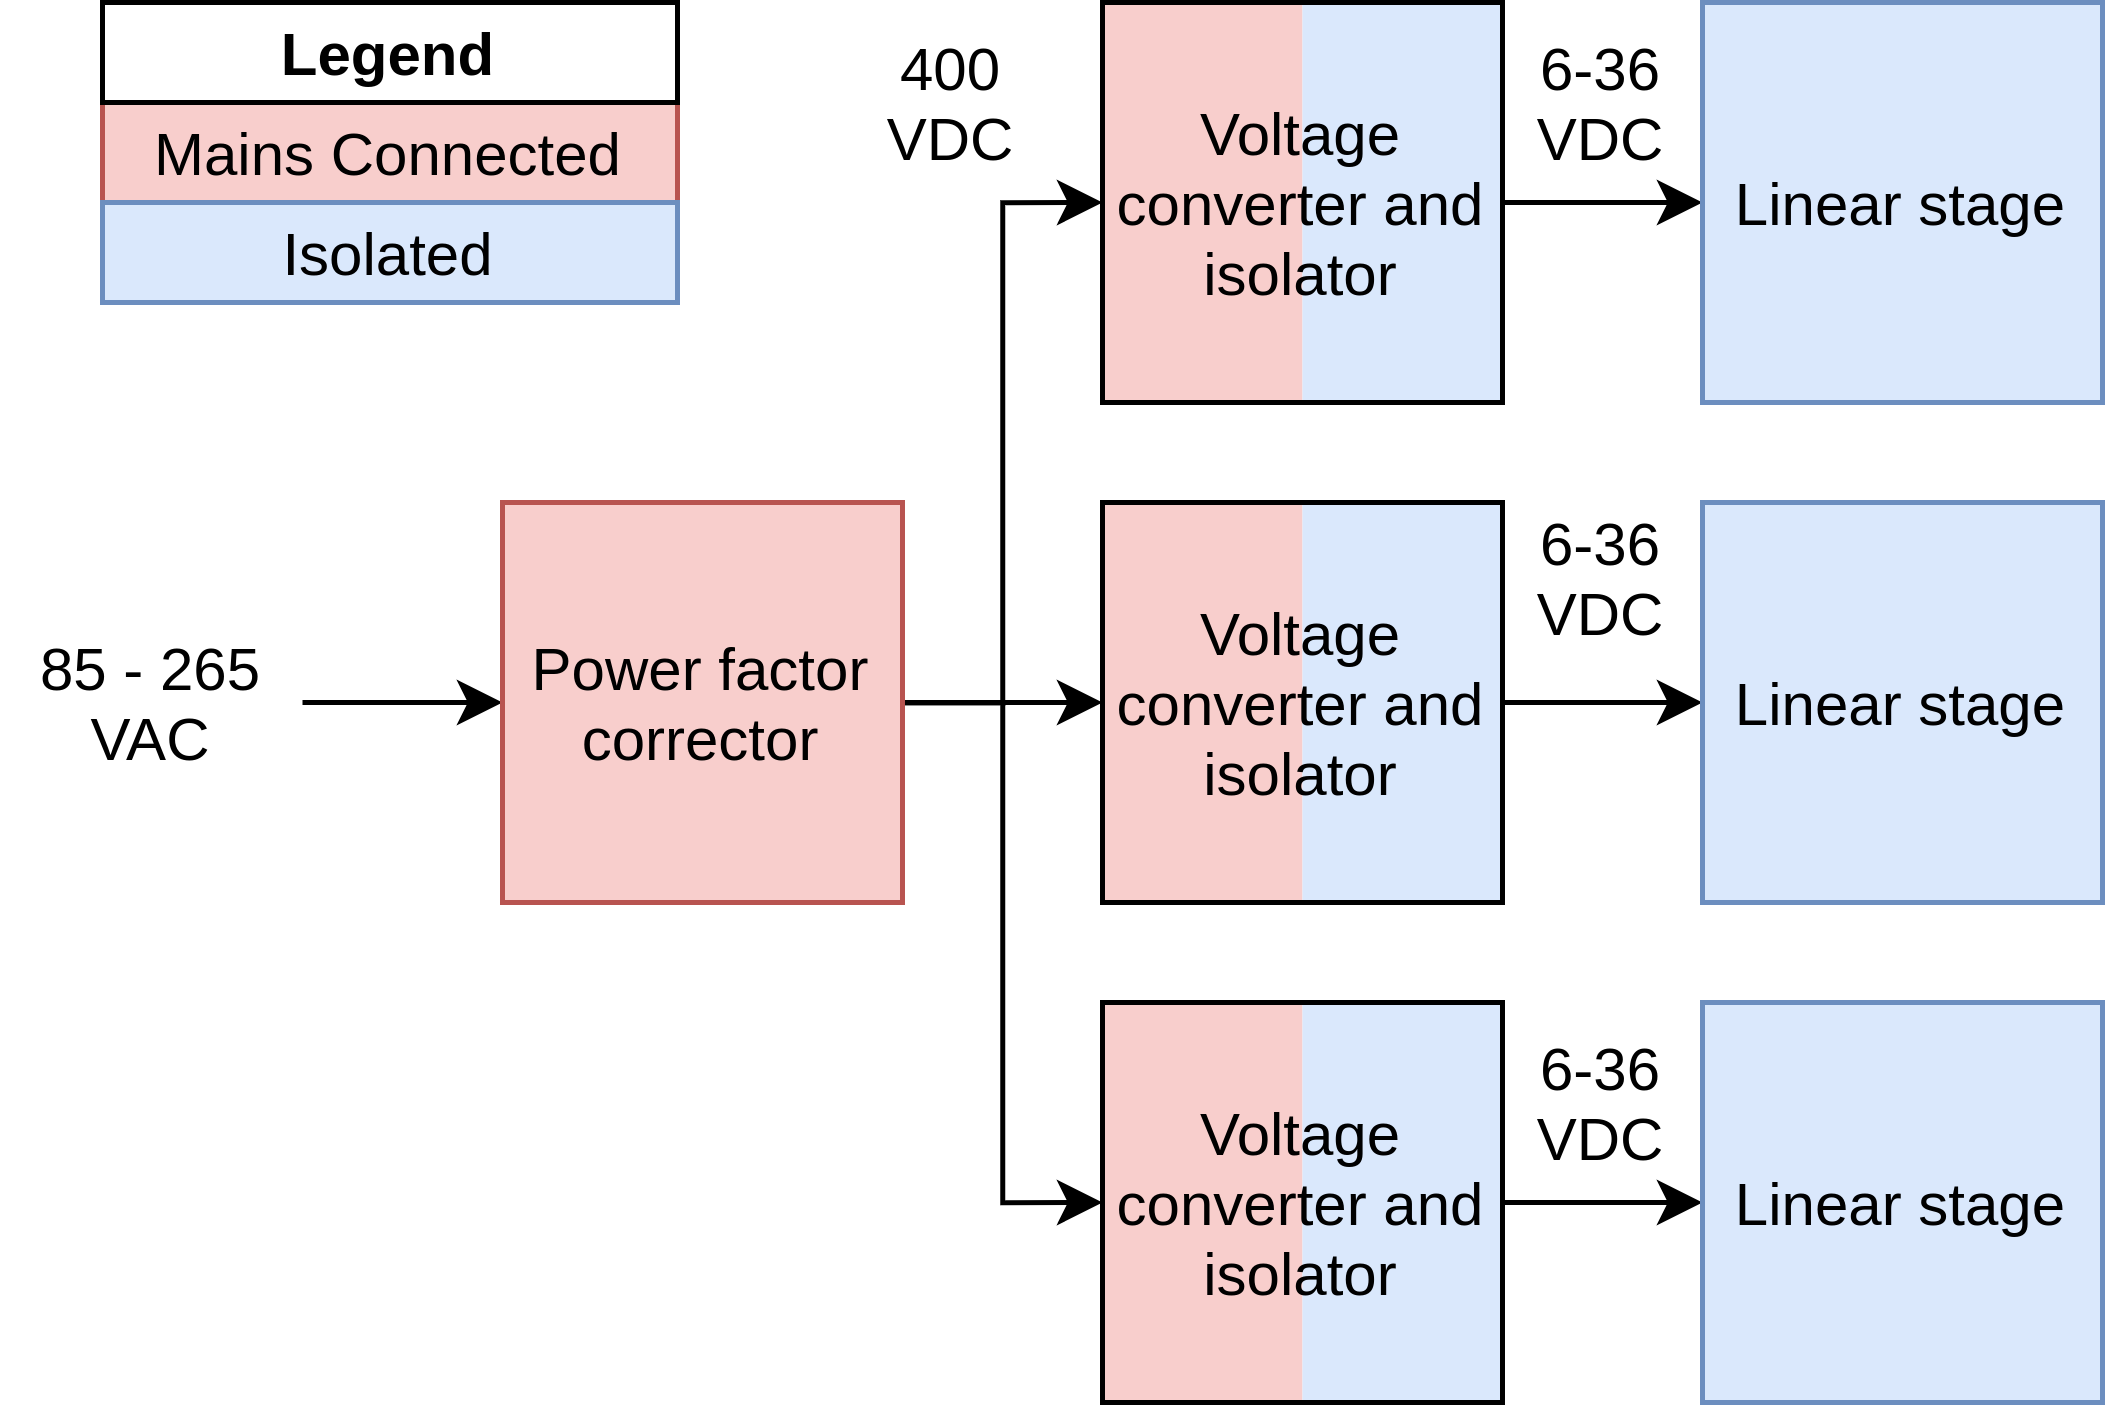
\includegraphics[width=0.8\textwidth]{acdctopo}
    \caption{AC to DC stage topology}
    \label{fig:acdctopo}
\end{figure}

\subsection{PFC stage  - Alex Jones}
\subsubsection{Requirements}
\begin{itemize}
\item 85-265 VAC input \begin{itemize}
    \item This is a widely accepted “universal” input range
\end{itemize}
\item 400 VDC output \begin{itemize}
    \item Common PFC designs rely on boost converters, requiring the intermediary design voltage to be higher than the maximum input voltage. Our 265 VAC input peaks at 370 volts, and this is increased to 400 volts nominally.
\end{itemize}
\item 600 watt total output \begin{itemize}
    \item Each channel can supply 150 watts, giving us a 450 watt total. 30 watts are added to each channel for the linear regulation. This leaves us at 540 watts. 600 watts was selected for some efficiency headroom and to prevent major voltage droops at full load.
\end{itemize}
\item 0.9 Power factor \begin{itemize}
    \item Not required in the US but the EU requires IEC 61000-3-2\cite{4} which wants power factor correction in all consumer devices. 
\end{itemize}
\end{itemize}


\subsubsection{Design}
PFC controller IC’s are available commercially. These frequently detail design equations for major components such as the primary inductor. Our selected controller is the BD7692FJ due to price and availability, as well as its thorough documentation allowing us to verify our design against known good equations. Its reference board is detailed thoroughly in \cite{1}. We selected a switching frequency of 500 kHz as this high frequency minimizes the size of inductors and filters needed, while not causing excessive switching losses in the cheaper range of diodes and MOSFETs. As the PFC resides before isolation, we opted to design a single PFC to supply all 3 channels rather than 3 independent PFCs. This choice was dictated by the availability and cost of appropriately sized PFC controllers.

The schematic of this PFC unit is in \autoref{fig:PFC}. Several values in this schematic are quite different from their ideal values in the name of BOM reduction, especially in the snubbers and filters where exact values are relatively unimportant. The passive components surrounding the MOSFET gate are very similar to the gate circuitry implemented on the isolation stage, and they are there to ensure proper startup function and MOSFET protection, which is critical in noisy inductive applications. A High cost portion in \autoref{fig:PFC} is the EMI filter. This was designed following the work of Mühlethaler et. al.\cite{8} as their paper details EMI filter design specifically for PFC units. This filter brings Vupiter into compliance with several standards, most notably IEC 61000-2-3 \cite{3} which focuses on the regulation of non-harmonic conduction back into mains. More work could be done on this filter for cost optimizations

One of the most critical components in any boost converter is the primary inductor. Due to the sinusoidal input and high desired output power, this inductor must tolerate extremely high peak currents. Our worst case of an 85 volt input generates a peak at approximately 20 amps. This far exceeds typical commercial inductor’s saturation limit, at least in our price range. Thus we are required to wind our inductor using ferrite cores. Erickson et. al.\cite{2} lays out a procedure for designing gapped inductors from commercially available cores. This procedure was followed to design the inductor used in these converters with cores purchased from Digikey. The core was wrapped with litz wire from ebay.

The PFC controller IC requires a supply voltage and has no provisions to efficiently bootstrap from the high input voltage. With efficiency as a design goal, classic Zener and resistor setups are unacceptable. Instead, we opt for a small offline converter based around the AP3917B. This regulator can be seen in \autoref{fig:buck}. The AP3917B is specifically designed for these offline applications as not only does it tolerate the high voltages but it can also drive its internal switch at extremely low duty cycles which is a key factor in such a large voltage transformation. The design of this converter is detailed thoroughly in a manufacturer application note in \cite{7}. With rough component values provided by those equations, the exact component selection came down once again to BOM reduction, trying to utilize as many of the same parts as the PFC circuitry. This converter is tuned for 15 volts and is also exported off-board to serve as a supply voltage for the control logic in the isolation stage, drastically improving their efficiency as well.

These two converters, the boost PFC and the offline buck go on one board, whose layout can be seen in \autoref{fig:pfclayout}. The buck converter is located along the bottom edge of the board, while the PFC module occupies the rest of the board. The EMI filter will either be placed in the currently unoccupied top left of the board or on a separate board. 

% The price for this board including the pcb itself, all the components, and the litz wire needed to wind the inductor comes out to 18 dollars.\\

\subsubsection{Performance}
Upon powering up the PFC board a flaw was discovered in the initial design. The secondary 15-volt converter used to power the logic had a dedicated rectifier that provided a path to ground that didn't pass through the current sense resistors. This meant that the controller could cause huge over-current events, saturating the inductor and destroying the MOSFET. In the prototype, this was fixed by replacing the 15-volt converter with a commercially available isolated 12-volt converter. Fixing this issue in a future revision would only require redesigning the buck converter to run off the output of the PFC stage, eliminating the need for a second rectifier.

Full testing of the board was not possible as the team had no access to a load rated at 400-volts that could take any appreciable percentage of the 600-watt output. The 400-volt output was confirmed with a multimeter. Noise measurements could not be taken reliably due to most oscilloscopes connection to earth ground.

\subsection{Isolation stage  - Alex Jones}
\subsubsection{Requirements}
\begin{itemize}
\item 400 VDC input \begin{itemize}
    \item This is coming from the PFC module, nominally 400 but we are designing for 380-420 actually
\end{itemize}
\item 36-6 VDC output \begin{itemize}
    \item The linear stage needs this variable output for efficiency and heat purposes. The board needs to automatically adjust to an input signal plus 6 volts. This 6 volts is the headroom the linear stage needs to both increase and decrease its output. This automatic adjustment should be highly bandwidth limited to prevent oscillations
\end{itemize}
\item 5.5 amp output \begin{itemize}
    \item Each channel can only supply 5 amps at any given voltage, and the additional 0.5 amps is allocated to supply all the auxiliary functions.

\end{itemize}
\item Full isolation \begin{itemize}
    \item This is important for both safety and functionality. The most notable standard requiring this isolation is IEC 62368 \cite{5}. From a functionality point of view, we want isolation so that we can use multiple channels in series for greater voltage ranges or as a bipolar supply.
\end{itemize}
\end{itemize}
\subsubsection{Design} 
For this design, we chose a two-switch forward converter, which has several advantages for this type of application. Firstly, being a buck-derived converter, the output inductor has a constant waveform through it, thus handling the majority of demand and reducing the need for costly and bulky capacitors. Secondly, the transformer design is simplified by the lack of any tertiary or reset windings such as in flyback converters. Third and possibly most critical, forward converters, unlike their resonant counterparts, can drastically vary their output range, whereas modern LLC converters would struggle to deviate from the designed voltage.  The pros and cons of various topologies are discussed more in-depth in Erickson et. al.\cite{2}.

Our converter is based around the NCP1252, chosen for its low cost and thorough documentation. As before, the manufacturer provides a document detailing the design of a reference board in \cite{9}. Our design has major deviations from this simple example, first and foremost in the isolated feedback section. This feedback network can be seen in \autoref{fig:forwardback} with a simplified version in \autoref{fig:forwardfeedbacksimp}. It has been complicated substantially from traditional designs due to the wide range of outputs this supply must generate. The optocoupler is powered from a regulated supply to ensure that the gain of the control loop is not impacted by the current output level. The feedback itself is managed by a differential amplifier to create the rather unique feedback plus volts effect.

\begin{figure}[H]
    \begin{center}
    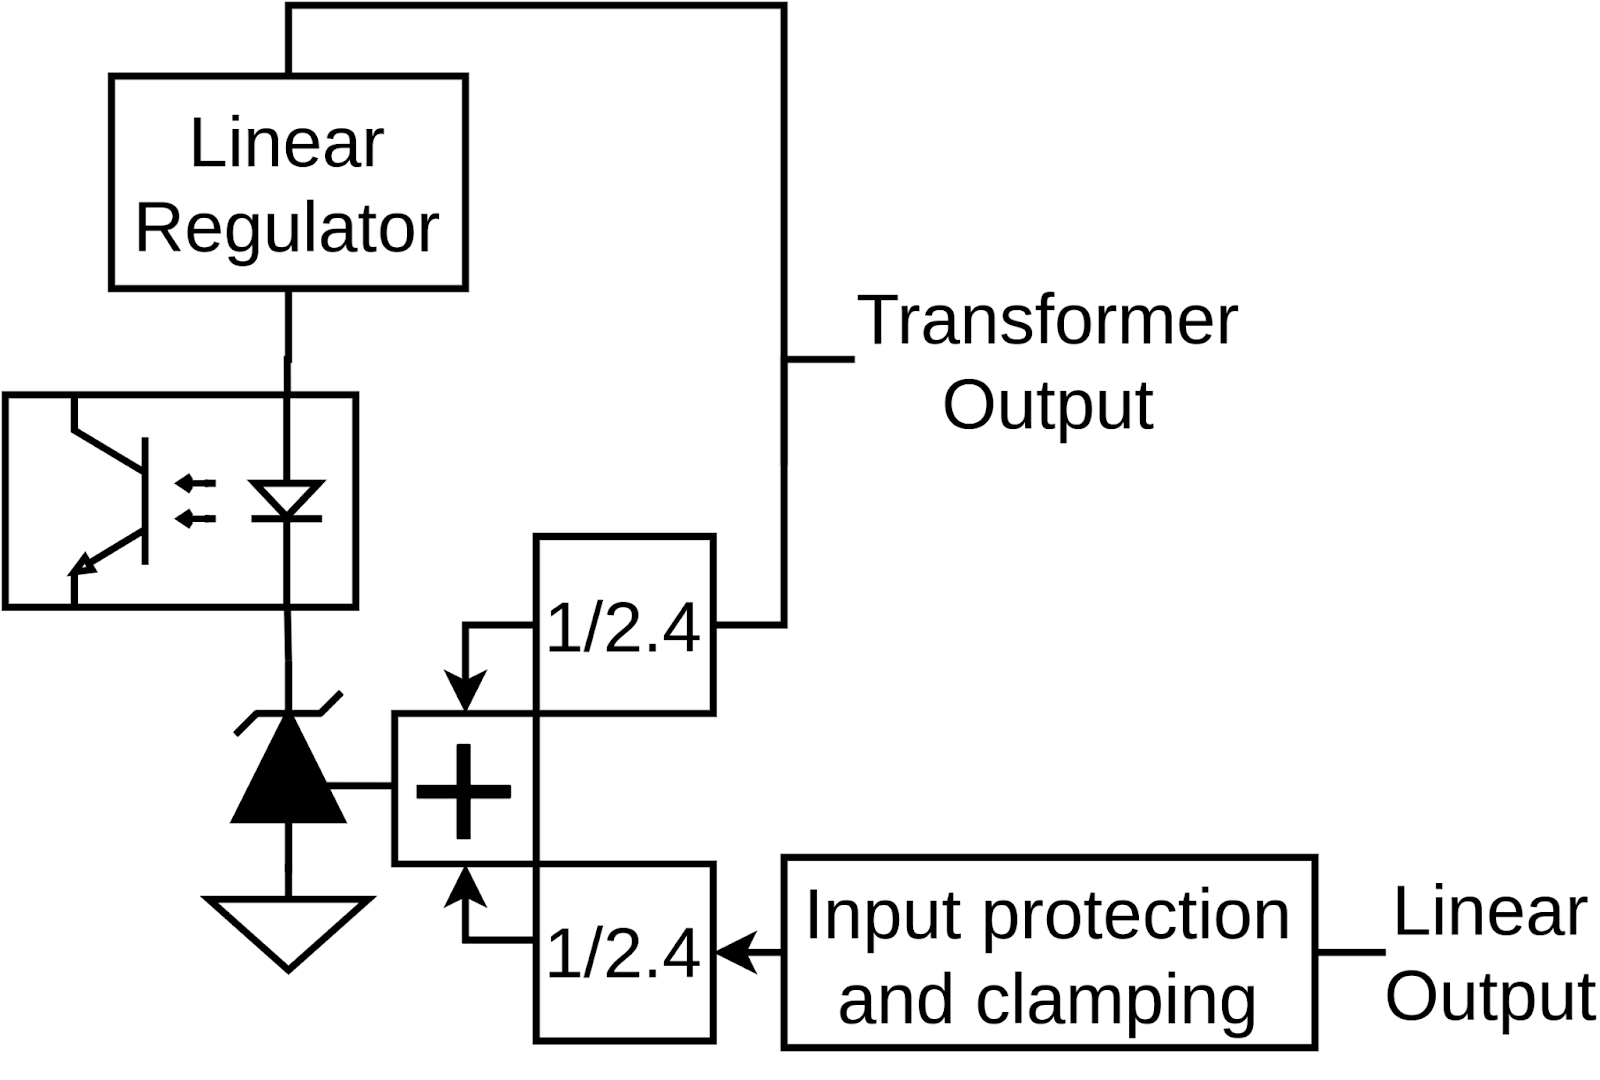
\includegraphics[width=0.4\textwidth]{forwardfeedbacksimp}
    \end{center}
    \caption{Complex feedback network for unique floating voltage operation}
    \label{fig:forwardfeedbacksimp}
\end{figure}

The bulk of the converter is in \autoref{fig:forwarddrive}. The gate driving is accomplished by a bootstrap gate driver IC, This driver generates the voltages needed for high-side driving of the N-channel MOSFETs used. This is both a cost and size reduction when compared with using a gate driver transformer. About 25\% of the components in the feedback section and this gate driver section are shared with the PFC board as a BOM reduction method.

The transformer used in \autoref{fig:forwarddrive} is custom-made and wound with litz wire, the same as the PFC inductor. Once again, Erickson et. al.’s\cite{2} procedure was used to design the transformer from commercially available cores. In addition to the insulation on the wires, polyimide tape will be added between the primary and secondary windings to add redundant isolation in accordance with IEC 62368\cite{5}.

These two sections reside on one board with a large gap in the ground plane for isolation. This layout is in \autoref{fig:forwardlay}. The gap between underneath the transformer and optocoupler exceeds IPC2221A\cite{6} creepage and clearance specifications by a factor of 2.

\subsubsection{Performance}
\label{sec:isoperformance}
Upon powering this board, two flaws were discovered. Firstly, the Zener diodes designed to protect the gate of the high side switch cause damage to the gate driver. Despite the gate driver being rated for the voltage, applying the 400 volts to the input with these diodes in place causes immediate decapsulation of the chip. 

The second error discovered was around the operation of the bootstrap gate driver. The majority of converters drive high and low side switches out of phase with one another. The on-state of the low switch provides a path through which the bootstrap capacitor can be pulled down and recharged. In our two-switch forward converter design, both switches need to switch simultaneously, and thus no discharge path exists. This was fixed by adding the red components in \autoref{fig:iso}. One of the two MOSFETs operates as an inverter while the other provides the path to ground.

\begin{figure}[H]
    \begin{center}
    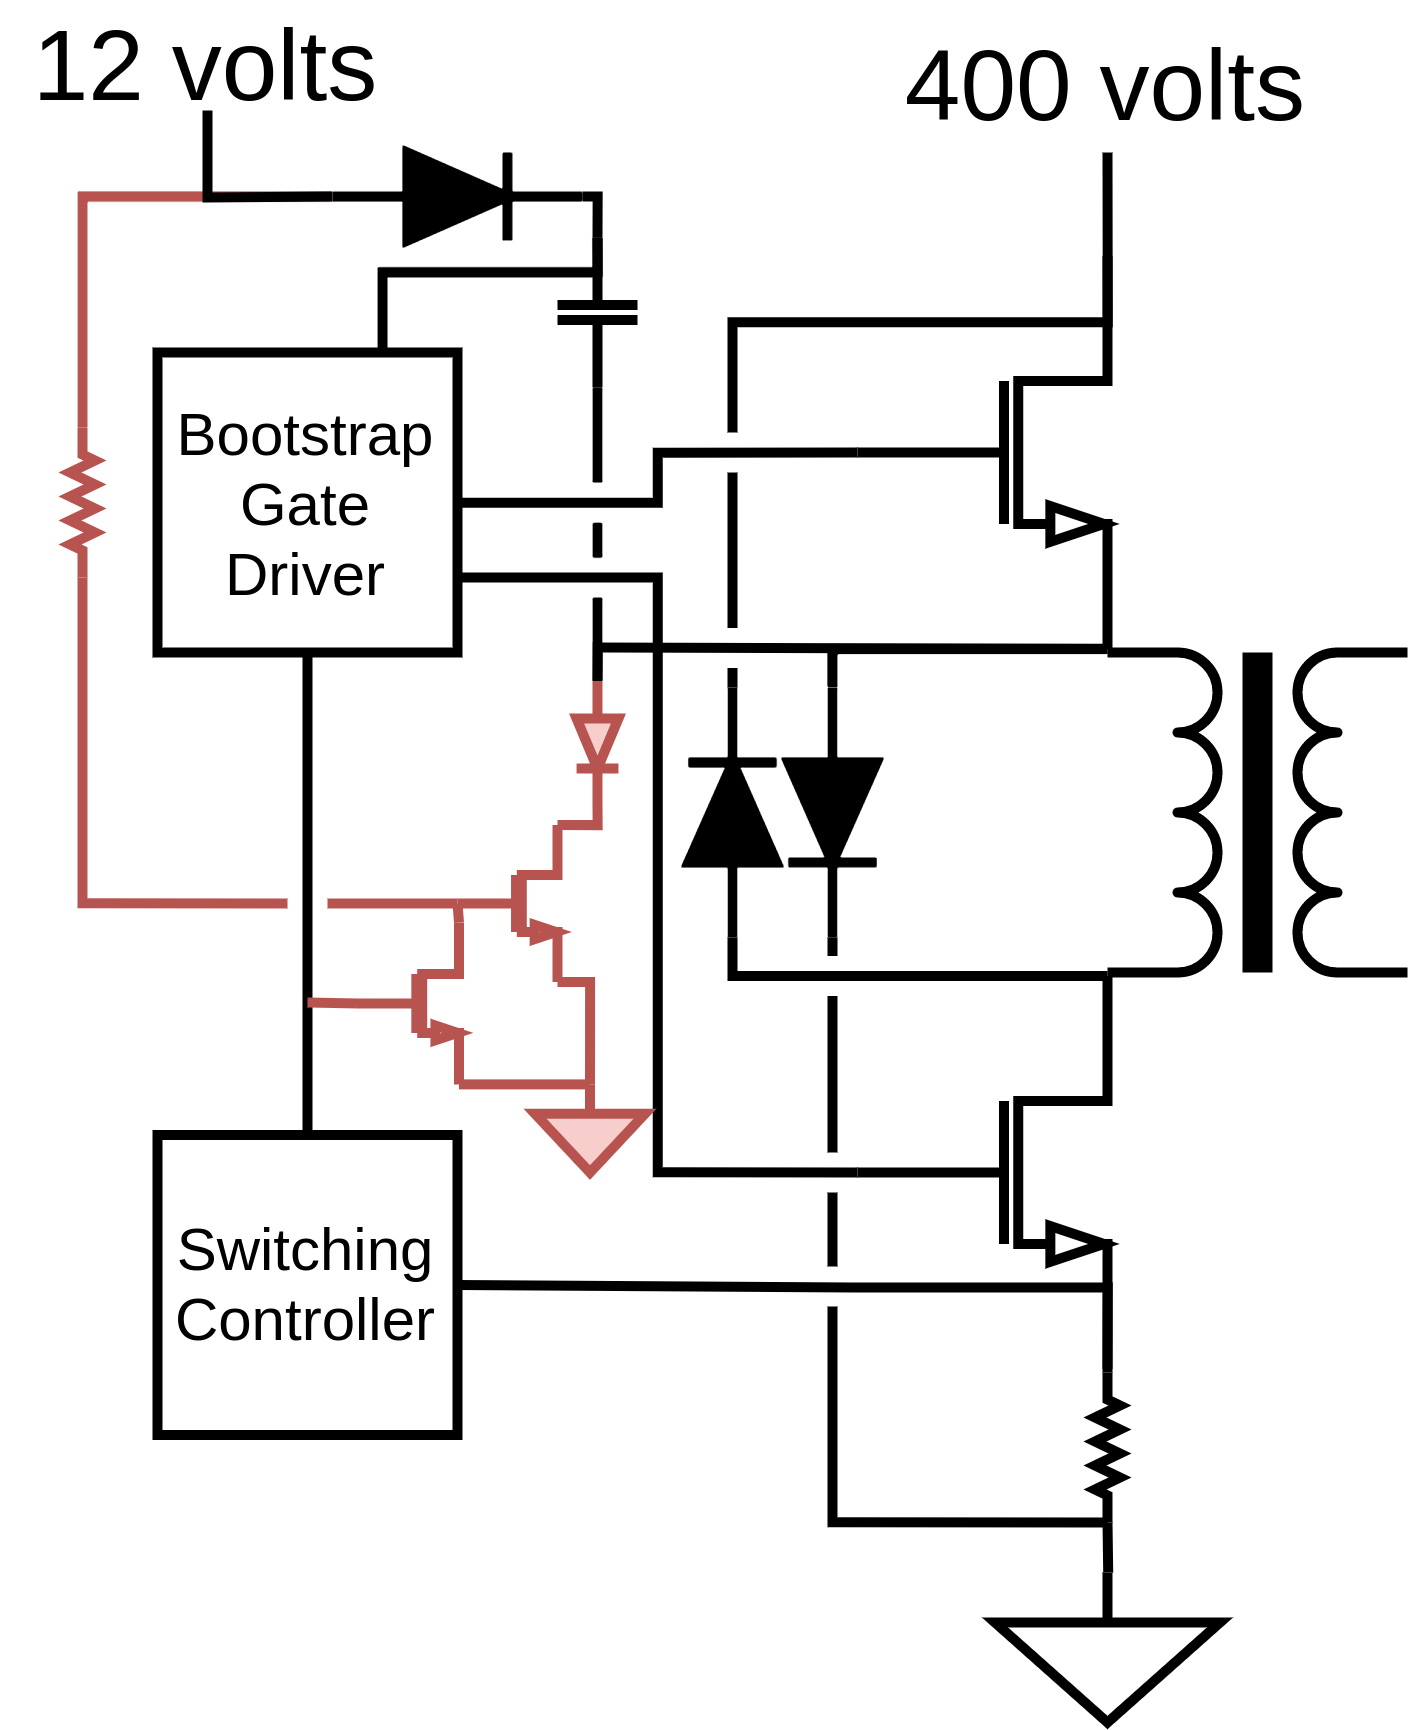
\includegraphics[width=0.4\textwidth]{iso}
    \end{center}
    \caption{Additional components needed for proper bootstrap operation}
    \label{fig:iso}
\end{figure}

With these two issues fixed, the board works for about 30 minutes. After those 30 minutes, there is an unresolved failure that occurred in both boards tested. This failure mode presents 2 volts on the output despite full 50\% duty cycle waveforms on the input. The culprit is believed to be the demagnetization diodes which if broken would leave the transformer in a saturated and a unable to transfer much energy. 

Future versions of this board would need to fix the longevity issues and improve the feedback network's bandwidth. The current version was designed with intentionally limited bandwidth to prevent minor fluctuations of the output of the linear stage from causing unnecessary changes in this converter's output. This bandwidth was limited right at the adjustable Zener's output, instead of at the linear board's feedback point like it should have been. This results in rather poor regulation when the board is working but is unrelated to the failures being seen.

\subsection{Computer Interface - Rice Shelley}
\begin{wrapfigure}[21]{r}{0.45\textwidth}
    \begin{center}
      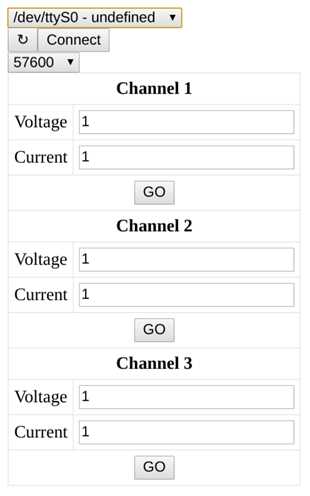
\includegraphics[width=0.43\textwidth]{computersoft.png}
    \end{center}
    \caption{Computer Graphical User Interface}
    \label{fig:computersoft}
  \end{wrapfigure}
The Vupiter DC power supply will have a computer interface supported by USB 2.0 and SCPI (Standard Commands for Programmable Instruments). The SCPI protocol will exist on top of the USB layer. The USB spec will be met with an FTDI chip that converts USB 2.0 to UART. The SCPI protocol interpreter is embedded into one of the power supply’s microcontrollers. The relatively simple SCPI protocol allows easy development of desktop software to control the power supply. The power supply will implement the DCPSUPPLY SCPI \cite{10}  base class to ensure basic compatibility with other SCPI power supply control software. An example of power supply control using SCPI is shown below. \\
\begin{verbatim}
*RST
INSTrument:NSELect 1
SOURce:VOLTage:LEVel:IMMediate:AMPLitude 12
OUTPut:STATe ON
\end{verbatim}

This SCPI command sequence would reset the power supply, select channel one, set the voltage to 12 volts, and then enable the output. In addition to the option to write control software using the SCPI interface, the user will be provided with desktop control software. The stock desktop control software is an application with an easy-to-use graphical user interface that can be used to set the voltage and current levels of the power supply. The stock control software can be seen in \autoref{fig:computersoft}.

\subsection{User Interface - Al Spies}
The user interface allows user to control device from front panel while viewing voltage and current readings from each channel of the power supply. Adjustments are made with encoders and variables can be viewed on 128 x 68 OLED display. User interface control is done with EFM8 board. User has option to Vupiter with a computer through communication to EFM8 board using UART and SCPI that are built into the design. Each channel of the power supply will have its own EFM8 board, encoders, and display. The EFM8 board coding was designed using Simplicity Studio software.
\begin{singlespace}
\noindent \textbf{Functions of EFM8}:
\vspace{-0.5cm}
\begin{itemize}
    \item Receive encoder signals \begin{itemize}
        \item Voltage encoder  \begin{itemize}
            \item Channel A
            \item Channel B
            \item Optional Button
        \end{itemize}
        \item Current encoder  \begin{itemize}
            \item Channel A
            \item Channel B
            \item Optional Button
        \end{itemize}
    \end{itemize}
    \item Receive analog signal from linear stage through onchip ADC \begin{itemize}
        \item Voltage
        \item Current
    \end{itemize}
    \item Send analog control signal to linear stage through onchip DAC \begin{itemize}
        \item Voltage
        \item Current
    \end{itemize}
    \item Send $I^2C$ control signals to OLED Display
    \item Communicate with UART board
\end{itemize}
\end{singlespace}
The user interface is expected to perform several tasks at the same time to control the system effectively. In order to achieve an effective program, interrupt routines are used for control of each task. Triggers for interrupts are done by either a timer for encoders and displays or input for UART when a signal is received. The flow chart in 
\autoref{fig:softflow} shows the method of control within the program.

\begin{figure}[H]
    \begin{center}
    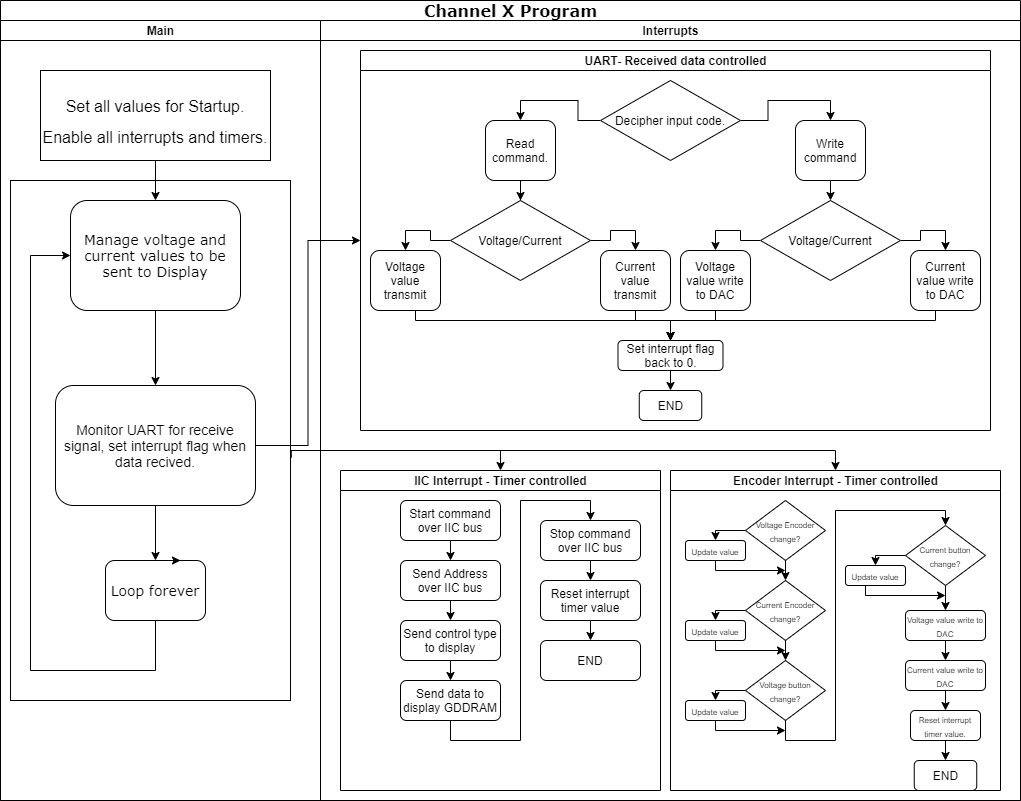
\includegraphics[width=0.7\textwidth]{softflow}
    \end{center}
    \caption{Flow chart of C program cycle and interrupts}
    \label{fig:softflow}
\end{figure}
\subsection{Budget - Al Spies}
In order to be competitive with market alternatives, the target cost was \$100. The initial targets for each subsection were: \$25 are for front panel display and button/knobs, \$50 for the power stages and PCBs, and \$25 for the casing of the supply. The final budget to create a power supply falls close to the initial goal, but total design cost with extra supplies and shipping cost drove the cost up to a range outside the initial goal. The final design project cost is approximately \$300, including all shipping expenses and resources used to build the prototype. \autoref{tab:costs} shows the breakdown of the cost to build an additional unit with all knowledge learned through the design and build process.

\begin{table}[H]
    \centering
    \begin{tabular}{| c | c | c | c |}
    \hline
     \textbf{Item} & \textbf{Cost} & \textbf{Quantity} & \textbf{Total}\\
     \hline
     PFC Board & \$18.00 & 1 & \$18.00\\ 
     Transformer Boards & \$8.00 & 3 & \$24.00\\  
     Linear Boards & \$6.00 & 3 & \$18.00\\
     Human Interface & \$6.00 & 3 & \$18.00\\
     OLED Displays & \$3.00 & 3 & \$9.00\\
     Case Material & \$16.00 & 1 & \$16.00\\
     \hline
     \hline
     Total & & &\$103.00\\
     \hline


    \end{tabular}
    \caption{Vupiter's build cost breakdown}
    \label{tab:costs}
\end{table}
\subsection{Case Construction - Al Spies}
A case may be used to house components of the system will be made out of two metal plates that are bent to dimensions 300mm x 300mm x 65mm when assembled together with a 3D printed front panel. Vent holes drilled manually in the sides for forced air-flow to keep the system within normal operating temperatures. The design is intended to be easily assembled so anyone can build with common tools of a household. Standards that apply to the device construction related to safety concerns are CFR §1500.49, IEC 62368, IEC 60950-1, and NFPA 70. The case was designed to meet these standards but never built as the SPaRC lab where Vupiter is staying is more than likely to take it apart and a case would only impede their efforts.
\pagebreak
\section{Summary - Al Spies}
There were a few complications through the build phase of the project but the completed prototype has two of the three circuit boards functioning as designed and the software interface performs as expected. The PFC board and linear boards perform well through testing but the isolation board only functions for some time before components fail. Some improvement to improve the longevity of the isolation stage is listed in \autoref{sec:isoperformance} Performance of the report. Other improvements to the design include:
\begin{singlespace}
\begin{itemize}
    \item Linear Board\begin{itemize}
        \item better microcontroller packageand pin remapping to avoid restraints of I/O
        \item multi-turn pots for ease of adjustments during calibration of circuits
        \item negative regulator for the negative op-amp rail
    \end{itemize}
    \item Transformer Board\begin{itemize}
        \item higher bandwidth feedback loop to improve regulation
        \item improved demagnetization diodes to prevent failures
        \item layout changes to improve minor component interference
    \end{itemize}
    \item PFC Board\begin{itemize}
    \item improved input filter to prevent conducted emissions 
    \item power buck regulator off of board's own output to remove extra rectifier
    \item 3 separate PFCs at 200 watt each rather than a single 600 watt for all three channels
    \end{itemize}
\end{itemize}
\end{singlespace}
With the exception of the isolation board issues, Vupiter performs well to design standard set at the beginning of the project. Testing on the PFC and linear boards work close to desired ranges and the interface performs as intended with intuitive design for users. The budget was maintained to a design standard, even though the prototype expenses were more than anticipated, and reproduction of the design is a cost-effective alternative to commercial products. The overall result of the Vupiter design is a success and provides a strong base for hobbies to build on.
\noindent


All files, including this report are hosted on our github:
\url{https://github.com/ams0187/Vupiter} Any file not reproduced here can be located there.
\pagebreak
\raggedright
\section{References}
\begingroup
\renewcommand{\section}[2]{}
\begin{thebibliography}{}
    \bibitem{expensive}
    Siglent Power Supplies, Siglent, Accessed 2021 [Online] Available: \url{
        https://siglentna.com/power-supplies/}
    \bibitem{adexpense}
    "High Performance Portable DC Bench Power Supply: Save Money and Free Up Bench Real Estate by Building Your Own", Analog Devices, July 2014 [Online] Available:
    \url{https://www.analog.com/media/en/technical-documentation/tech-articles/lt-journal-article/LTJournal-V24N2-02-df-BenchSupply-Szolusha.pdf}
    \bibitem{1} 
    “Boundary Current Mode Method 200 W 400 V BD7692FJ Reference Board ,” 2019. [Online]. Available: \url{https://fscdn.rohm.com/en/products/databook/applinote/ic/power/acdc_converter/bd7692fj-evk-001_ug-e.pdf}

    \bibitem{2} 
    R. W. Erickson and Maksimovic Dragan, Fundamentals of power electronics. New York, New York: Springer Science + Business Media, 2012.

    \bibitem{3}
    IEC, “Description of the environment - Radiated and non-network-frequency-related conducted phenomena,” IEC Webstore, 1992. [Online]. Available: 
    \url{https://webstore.iec.ch/publication/4134}

    \bibitem{4}
    IEC, “Electromagnetic compatibility (EMC) - Part 3-2: Limits - Limits for harmonic current emissions (equipment input current 16 A per phase),” IEC Webstore, 2018. [Online]. Available:
    \url{https://webstore.iec.ch/publication/28164}

    \bibitem{aoe}
    Horowitz, P., \&; Hill, W. (2020). The art of electronics: The x-chapters. In The art of electronics: The x-chapters (p. 225). Cambridge, United Kingdom: Cambridge University Press.

    \bibitem{5}
    IEC, “Audio/video, information and communication technology equipment - Part 1: Safety requirements,” IEC Webstore, 2018. [Online]. Available: 
    \url{https://webstore.iec.ch/publication/27412}

    \bibitem{796} UL, "Printed Wiring Boards," UL Standards Site, Revised 2020. [Online]. Available: \url{https://standardscatalog.ul.com/ProductDetail.aspx?productId=UL796}

    \bibitem{6}
    IEC, “Generic Standard on Printed Board Design” IPC, 2003. [Online]. Available: \url{https://www.ipc.org/TOC/IPC-2221A.pdf}

    \bibitem{7}
    “1.44W AP3917B EV1 Evaluation Board User’s Guide,” Diodes Incorporated, 20-Feb-2020. [Online]. Available: \url{https://www.diodes.com/assets/Evaluation-Boards/1.44W-AP3917B-Single-Output-12V-120mA-EV1-User-Guide-Rev-1.1-Eval-Board-User-Guide.pdf}

    \bibitem{8}
    J. Mühlethaler et. al., “Optimal design of EMI filters for single-phase boost PFC circuits,” IEEE Xplore, 2012. [Online]. Available: 
    \url{https://ieeexplore.ieee.org/document/6388754}
    \bibitem{9}
    “AND8373/D - 2 Switch-Forward Current Mode Converter,” 2010. [Online]. Available: \url{https://www.onsemi.com/pub/collateral/and8373-d.pdf}

    \bibitem{10}
    “Standard Commands for Programmable Instruments (SCPI) - Volume 1: Syntax and Style,” IVI Foundation, 1999. [Online]. Available: \url{https://www.ivifoundation.org/docs/scpi-99.pdf}

    \bibitem{11}
    “16 CFR § 1500.49 - Technical requirements for determining a sharp metal or glass edge in toys and other articles intended for use by children under 8 years of age.,” Legal Information Institute. [Online]. Available: \url{https://www.law.cornell.edu/cfr/text/16/1500.49}
    
    \bibitem{12}
    “NFPA 70,” NFPA 70®: National Electrical Code®. [Online]. Available: \url{https://www.nfpa.org/codes-and-standards/all-codes-and-standards/list-of-codes-and-standards/detail?code=70.} 
    
    \bibitem{13}
    IEC, “Electromagnetic compatibility (EMC) - Part 3-2: Limits - Limits for harmonic current emissions (equipment input current 16 A per phase),” IEC Webstore, 2005. [Online]. Available:
    \url{https://webstore.iec.ch/publication/4024}
\end{thebibliography}
\endgroup
\pagebreak
\section{Appendices}
\subsection{Appendix A - Team Organization}
Alex Jones worked as team lead and on the design and debugging of all three boards. Chase Flatau worked on debugging, layout, assembly, and testing of the boards. Al Spies and Rice Shelley collaborated closely on the design and implementation of the software involved in both the computer and physical interfaces.

\subsection{Appendix B - Linear board sources}

\begin{figure}[H]
    \centering
    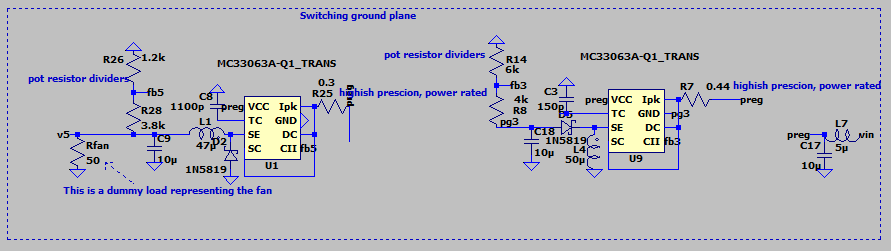
\includegraphics[width=0.8\textwidth]{chase2}
    \caption{Switching Section of the Linear Board}
    \label{fig:chase2}
\end{figure}


\begin{figure}[H]
    \centering
    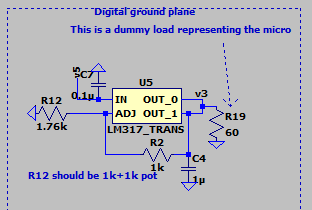
\includegraphics[width=0.8\textwidth]{chase3}
    \caption{Linear Regulator for micro controller of the Linear Board}
    \label{fig:chase3}
\end{figure}

\begin{figure}[H]
    \centering
    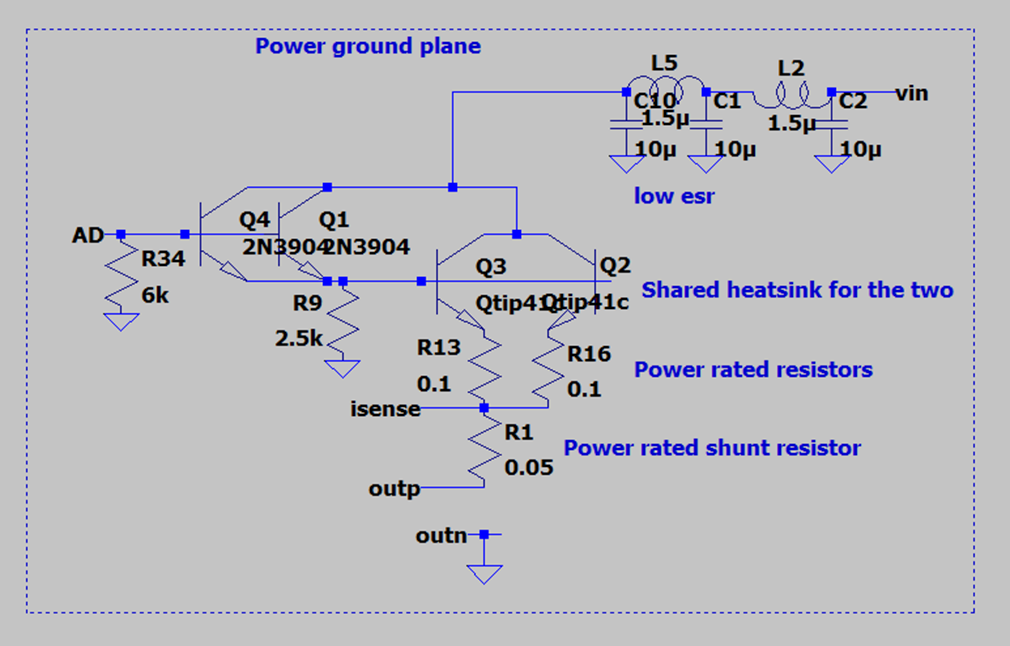
\includegraphics[width=0.8\textwidth]{chase4}
    \caption{Power Section of the Linear Board}
    \label{fig:chase4}
\end{figure}

\begin{figure}[H]
    \centering
    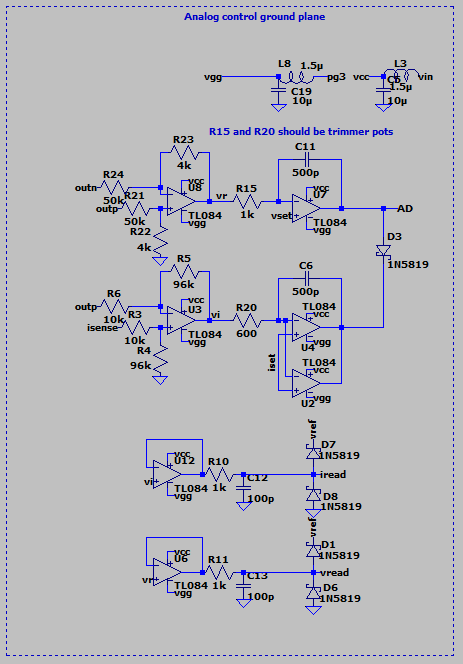
\includegraphics[width=0.6\textwidth]{chase5}
    \caption{Analog Control Section of the Linear Board}
    \label{fig:chase5}
\end{figure}

\begin{figure}[H]
    \centering
    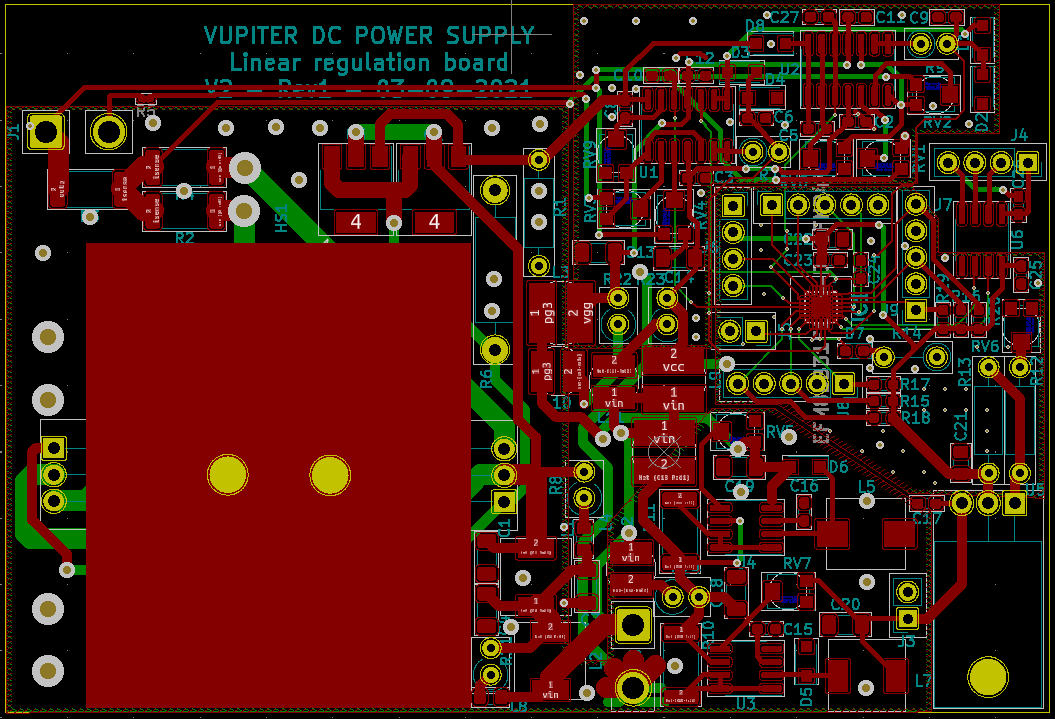
\includegraphics[width=0.8\textwidth]{chase6}
    \caption{Linear Board Design}
    \label{fig:chase6}
\end{figure}
% \csvautolongtable[table head=\hline
% \csvlinetotablerow\\\hline
% \endfirsthead\hline
% \csvlinetotablerow\\\hline
% \endhead\hline
% \caption{Linear Board Bill of Materials}
% \label{app:brdbom}
% \endfoot,
% respect all
% ]{brd.csv}
\subsection{Appendix C - PFC board sources}

\begin{figure}[H]
    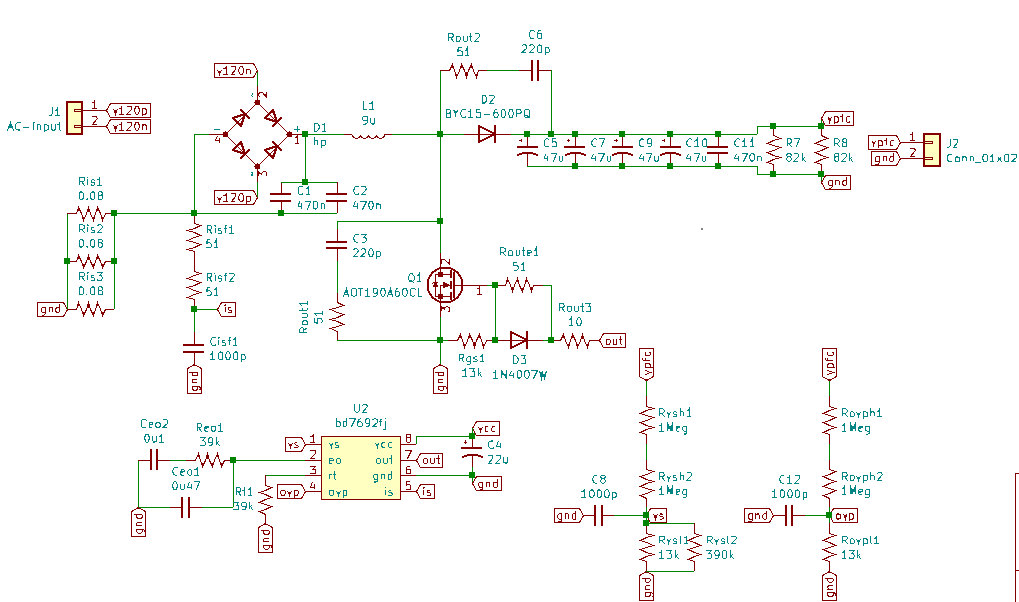
\includegraphics[width=\textwidth]{pfcschema}
    \caption{PFC converter schematic}
    \label{fig:PFC}
\end{figure}

\begin{figure}[H]
    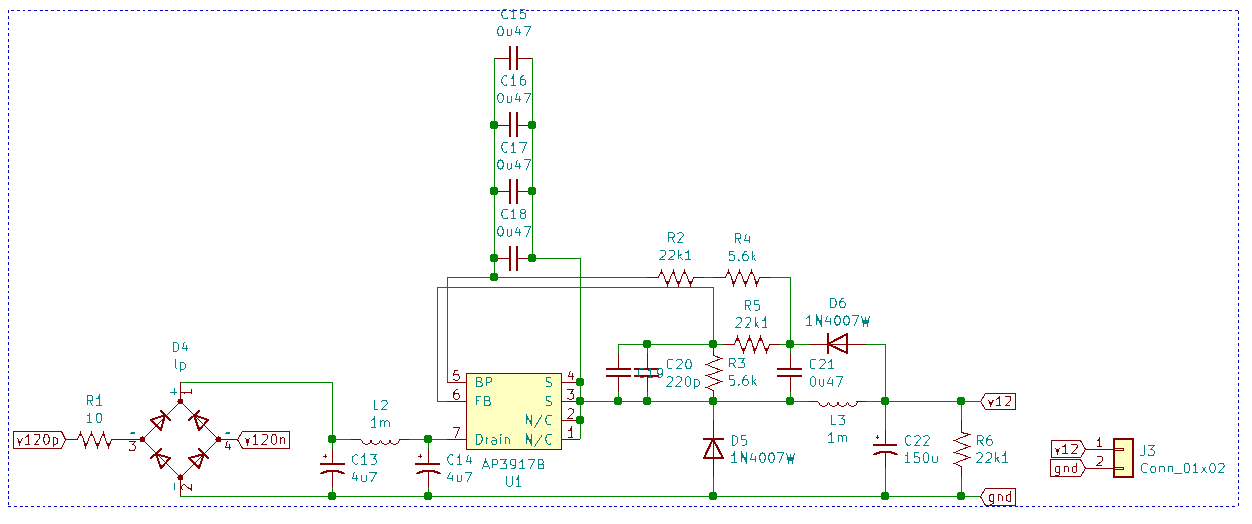
\includegraphics[width=\textwidth]{pfcbuck}
    \caption{15 volt offline buck converter design}
    \label{fig:buck}
\end{figure}

\begin{figure}[H]
    \centering
        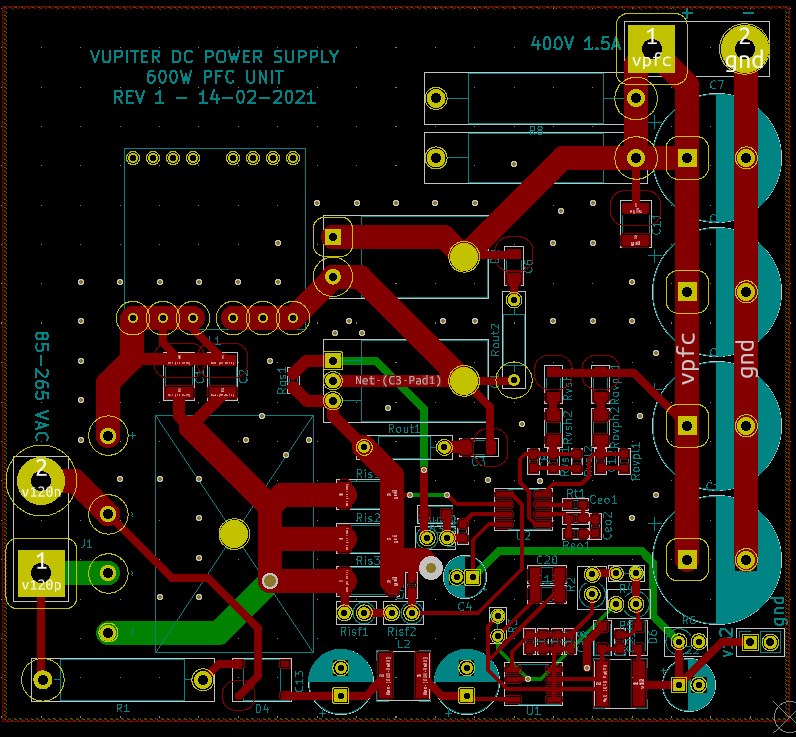
\includegraphics[width=0.75\textwidth]{pfclayout}
        \caption{PFC board layout}
        \label{fig:pfclayout}
    \centering
\end{figure}
% \csvautolongtable[table head=\hline
% \csvlinetotablerow\\\hline
% \endfirsthead\hline
% \csvlinetotablerow\\\hline
% \endhead\hline
% \caption{PFC Board Bill of Materials}
% \label{app:pfcbom}
% \endfoot,
% respect all
% ]{pfc.csv}

\subsection{Appendix D - Isolation board sources}

\begin{figure}[H]
    \centering
    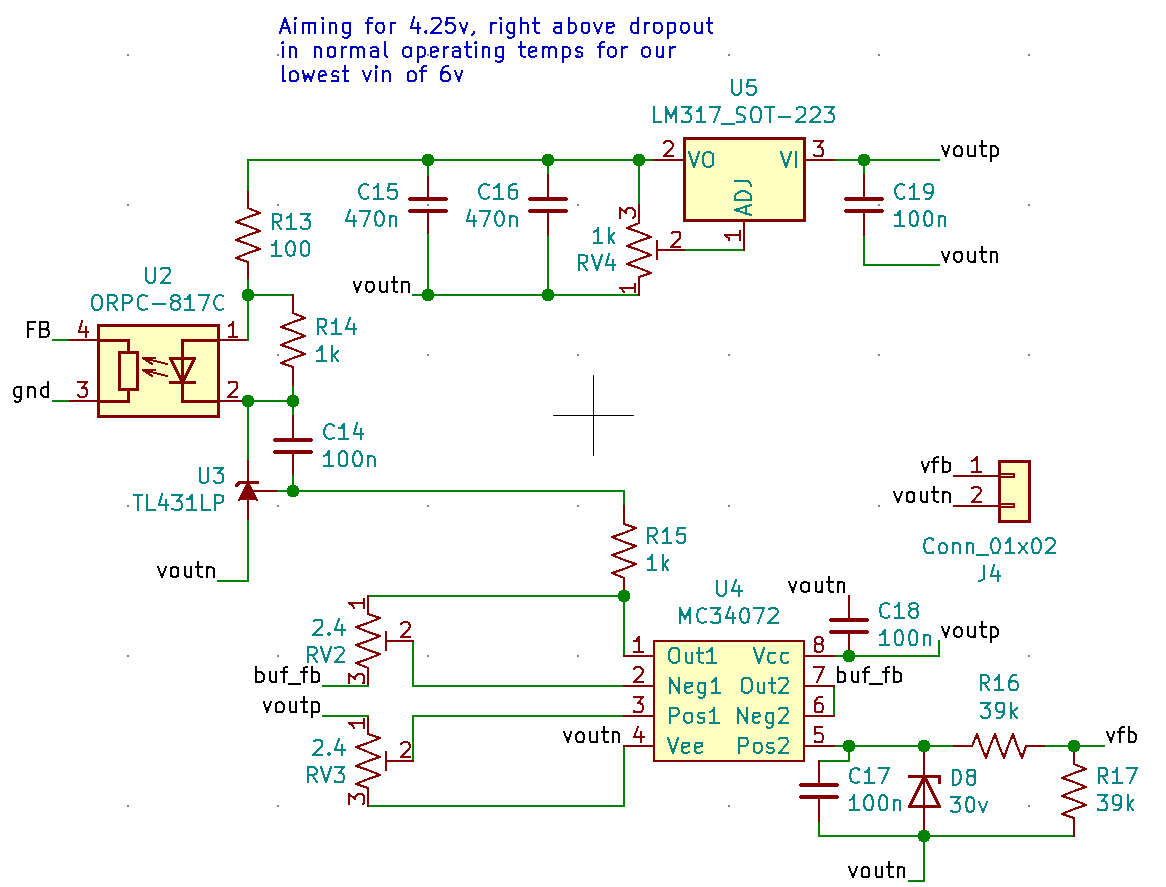
\includegraphics[width=0.5\textwidth]{forwardfeedback}
    \caption{Isolated feedback drive}
    \label{fig:forwardback}
\end{figure}
\begin{figure}[H]
    \centering
    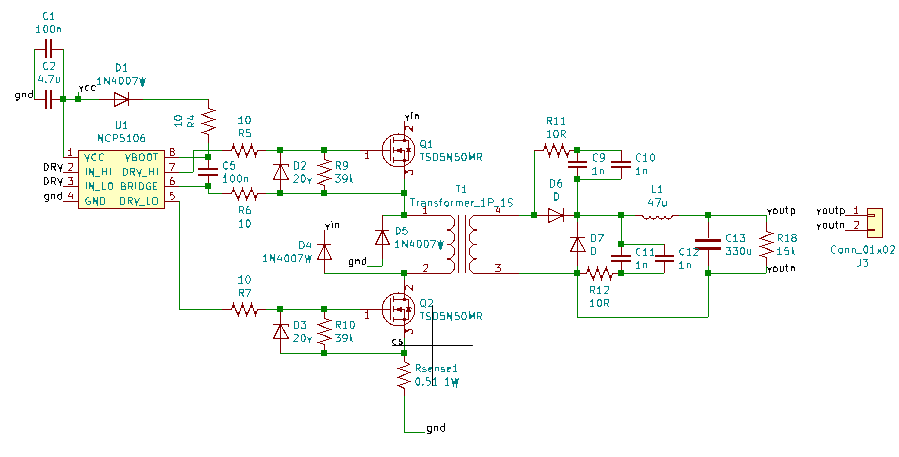
\includegraphics[width=0.75\textwidth]{forwarddrive}
    \caption{Forward converter design}
    \label{fig:forwarddrive}
\end{figure}
\begin{figure}[H]
    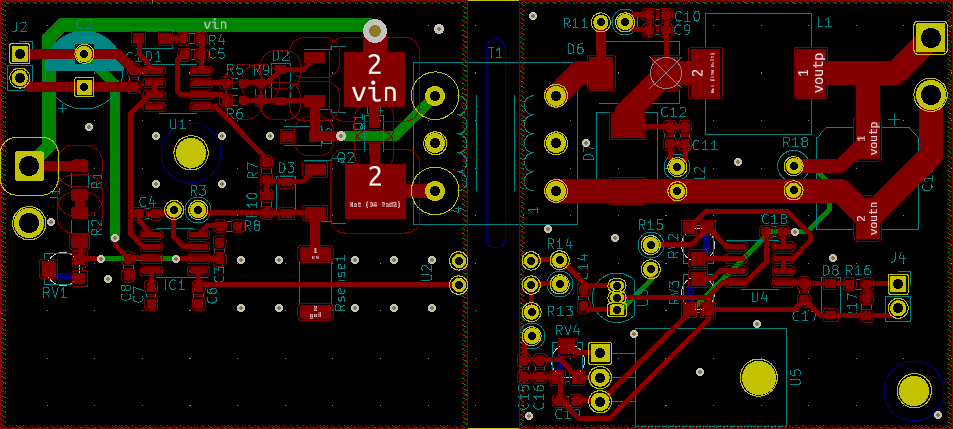
\includegraphics[width=\textwidth]{forwardlayout}
    \caption{Forward converter design}
    \label{fig:forwardlay}
\end{figure}

% \csvautolongtable[table head=\hline
% \csvlinetotablerow\\\hline
% \endfirsthead\hline
% \csvlinetotablerow\\\hline
% \endhead\hline
% \caption{Isolation Board Bill of Materials}
% \label{app:isobom}
% \endfoot,
% respect all
% ]{iso.csv}


\end{document}